\documentclass[twoside]{article}

% Packages required by doxygen
\usepackage{fixltx2e}
\usepackage{calc}
\usepackage{doxygen}
\usepackage[export]{adjustbox} % also loads graphicx
\usepackage{graphicx}
\usepackage[utf8]{inputenc}
\usepackage{makeidx}
\usepackage{multicol}
\usepackage{multirow}
\PassOptionsToPackage{warn}{textcomp}
\usepackage{textcomp}
\usepackage[nointegrals]{wasysym}
\usepackage[table]{xcolor}

% NLS support packages
\usepackage[ngerman]{babel}

% Font selection
\usepackage[T1]{fontenc}
\usepackage[scaled=.90]{helvet}
\usepackage{courier}
\usepackage{amssymb}
\usepackage{sectsty}
\renewcommand{\familydefault}{\sfdefault}
\allsectionsfont{%
  \fontseries{bc}\selectfont%
  \color{darkgray}%
}
\renewcommand{\DoxyLabelFont}{%
  \fontseries{bc}\selectfont%
  \color{darkgray}%
}
\newcommand{\+}{\discretionary{\mbox{\scriptsize$\hookleftarrow$}}{}{}}

% Page & text layout
\usepackage{geometry}
\geometry{%
  a4paper,%
  top=2.5cm,%
  bottom=2.5cm,%
  left=2.5cm,%
  right=2.5cm%
}
\tolerance=750
\hfuzz=15pt
\hbadness=750
\setlength{\emergencystretch}{15pt}
\setlength{\parindent}{0cm}
\setlength{\parskip}{0.2cm}
\makeatletter
\renewcommand{\paragraph}{%
  \@startsection{paragraph}{4}{0ex}{-1.0ex}{1.0ex}{%
    \normalfont\normalsize\bfseries\SS@parafont%
  }%
}
\renewcommand{\subparagraph}{%
  \@startsection{subparagraph}{5}{0ex}{-1.0ex}{1.0ex}{%
    \normalfont\normalsize\bfseries\SS@subparafont%
  }%
}
\makeatother

% Headers & footers
\usepackage{fancyhdr}
\pagestyle{fancyplain}
\fancyhead[LE]{\fancyplain{}{\bfseries\thepage}}
\fancyhead[CE]{\fancyplain{}{}}
\fancyhead[RE]{\fancyplain{}{\bfseries\leftmark}}
\fancyhead[LO]{\fancyplain{}{\bfseries\rightmark}}
\fancyhead[CO]{\fancyplain{}{}}
\fancyhead[RO]{\fancyplain{}{\bfseries\thepage}}
\fancyfoot[LE]{\fancyplain{}{}}
\fancyfoot[CE]{\fancyplain{}{}}
\fancyfoot[RE]{\fancyplain{}{\bfseries\scriptsize Erzeugt am Fre Apr 29 2016 17\+:04\+:13 für μ\+Crypt\+Lib von Doxygen }}
\fancyfoot[LO]{\fancyplain{}{\bfseries\scriptsize Erzeugt am Fre Apr 29 2016 17\+:04\+:13 für μ\+Crypt\+Lib von Doxygen }}
\fancyfoot[CO]{\fancyplain{}{}}
\fancyfoot[RO]{\fancyplain{}{}}
\renewcommand{\footrulewidth}{0.4pt}
\renewcommand{\sectionmark}[1]{%
  \markright{\thesection\ #1}%
}

% Indices & bibliography
\usepackage{natbib}
\usepackage[titles]{tocloft}
\setcounter{tocdepth}{3}
\setcounter{secnumdepth}{5}
\makeindex

% Hyperlinks (required, but should be loaded last)
\usepackage{ifpdf}
\ifpdf
  \usepackage[pdftex,pagebackref=true]{hyperref}
\else
  \usepackage[ps2pdf,pagebackref=true]{hyperref}
\fi
\hypersetup{%
  colorlinks=true,%
  linkcolor=blue,%
  citecolor=blue,%
  unicode%
}

% Custom commands
\newcommand{\clearemptydoublepage}{%
  \newpage{\pagestyle{empty}\cleardoublepage}%
}


%===== C O N T E N T S =====

\begin{document}

% Titlepage & ToC
\hypersetup{pageanchor=false,
             bookmarks=true,
             bookmarksnumbered=true,
             pdfencoding=unicode
            }
\pagenumbering{roman}
\begin{titlepage}
\vspace*{7cm}
\begin{center}%
{\Large μ\+Crypt\+Lib \\[1ex]\large 0.\+1 }\\
\vspace*{1cm}
{\large Erzeugt von Doxygen 1.8.9.1}\\
\vspace*{0.5cm}
{\small Fre Apr 29 2016 17:04:13}\\
\end{center}
\end{titlepage}
\tableofcontents
\pagenumbering{arabic}
\hypersetup{pageanchor=true}

%--- Begin generated contents ---
\section{Klassen-\/\+Verzeichnis}
\subsection{Auflistung der Klassen}
Hier folgt die Aufzählung aller Klassen, Strukturen, Varianten und Schnittstellen mit einer Kurzbeschreibung\+:\begin{DoxyCompactList}
\item\contentsline{section}{\hyperlink{classuCrypt_1_1uCryptLib}{u\+Crypt\+::u\+Crypt\+Lib} \\*Part of a Cryptography Library that\textquotesingle{}s built to make encryption and decryption as easy and fast as possible for third party tools }{\pageref{classuCrypt_1_1uCryptLib}}{}
\end{DoxyCompactList}

\section{Klassen-\/\+Dokumentation}
\hypertarget{classuCrypt_1_1uCryptLib}{}\subsection{u\+Crypt\+:\+:u\+Crypt\+Lib Klassenreferenz}
\label{classuCrypt_1_1uCryptLib}\index{u\+Crypt\+::u\+Crypt\+Lib@{u\+Crypt\+::u\+Crypt\+Lib}}


The \hyperlink{classuCrypt_1_1uCryptLib}{u\+Crypt\+Lib} class is part of a Cryptography Library that\textquotesingle{}s built to make encryption and decryption as easy and fast as possible for third party tools.  




{\ttfamily \#include $<$u\+Crypt\+Lib.\+h$>$}



Zusammengehörigkeiten von u\+Crypt\+:\+:u\+Crypt\+Lib\+:\nopagebreak
\begin{figure}[H]
\begin{center}
\leavevmode
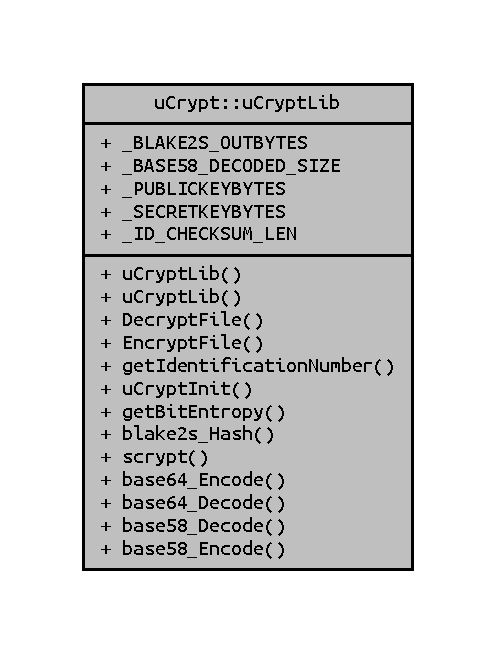
\includegraphics[width=238pt]{classuCrypt_1_1uCryptLib__coll__graph}
\end{center}
\end{figure}
\subsubsection*{Öffentliche Methoden}
\begin{DoxyCompactItemize}
\item 
\hypertarget{classuCrypt_1_1uCryptLib_aab8ae866a5f5bb7728b76a217f7cabf0}{}\hyperlink{classuCrypt_1_1uCryptLib_aab8ae866a5f5bb7728b76a217f7cabf0}{u\+Crypt\+Lib} ()\label{classuCrypt_1_1uCryptLib_aab8ae866a5f5bb7728b76a217f7cabf0}

\begin{DoxyCompactList}\small\item\em \hyperlink{classuCrypt_1_1uCryptLib}{u\+Crypt\+Lib} Default-\/\+Konstruktor \end{DoxyCompactList}\item 
\hyperlink{classuCrypt_1_1uCryptLib_a87345999d9b68b3e116e091f5d5b1e80}{u\+Crypt\+Lib} (std\+::string e\+Mail, std\+::string passwd)
\begin{DoxyCompactList}\small\item\em \hyperlink{classuCrypt_1_1uCryptLib}{u\+Crypt\+Lib} Konstruktor, welcher sofort eine Initialisierung durchführt. \end{DoxyCompactList}\item 
uint8\+\_\+t \hyperlink{classuCrypt_1_1uCryptLib_a868127bd1d2aa4edd62076663d801b66}{Decrypt\+File} (std\+::string file\+Name, std\+::string source\+Path, std\+::string target\+Path=\char`\"{}\char`\"{})
\begin{DoxyCompactList}\small\item\em Decrypt\+File Decryptfile führt die Entschlüsselung der Datei durch. \end{DoxyCompactList}\item 
uint8\+\_\+t \hyperlink{classuCrypt_1_1uCryptLib_a2a5e702b03339e4d1f15b8fbbf67e635}{Encrypt\+File} (std\+::string file\+Name, std\+::string source\+Path, std\+::string recipient\+I\+Ds\mbox{[}$\,$\mbox{]}, uint8\+\_\+t num\+Recipients, std\+::string target\+Path=\char`\"{}\char`\"{})
\begin{DoxyCompactList}\small\item\em Encrypt\+File Encrypt\+File führt die Verschlüsselung der Datei durch. \end{DoxyCompactList}\item 
std\+::string \hyperlink{classuCrypt_1_1uCryptLib_a6a659692c488ec460fa123ad81fa46f1}{get\+Identification\+Number} ()
\begin{DoxyCompactList}\small\item\em get\+Identification\+Number get\+Identification\+Number gibt die Variable \+\_\+identification\+Number zurück. \end{DoxyCompactList}\item 
void \hyperlink{classuCrypt_1_1uCryptLib_a6d7c6328bb218876de708d43be91494d}{u\+Crypt\+Init} (std\+::string e\+Mail, std\+::string passwd)
\begin{DoxyCompactList}\small\item\em u\+Crypt\+Init Die Methode u\+Crypt\+Init führt eine Initialisierung durch. \end{DoxyCompactList}\end{DoxyCompactItemize}
\subsubsection*{Öffentliche, statische Methoden}
\begin{DoxyCompactItemize}
\item 
static double \hyperlink{classuCrypt_1_1uCryptLib_af460e066f8c91c19d70306efdd7704b3}{get\+Bit\+Entropy} (std\+::string s)
\begin{DoxyCompactList}\small\item\em get\+Bit\+Entropy Die Methode get\+Bit\+Entropy überprüft den String auf seine Bit Entropie. \end{DoxyCompactList}\item 
static int \hyperlink{classuCrypt_1_1uCryptLib_a72b831c97eb1fc974ad32a63931de4d3}{blake2s\+\_\+\+Hash} (uint8\+\_\+t $\ast$out, const void $\ast$in, const void $\ast$key, const uint8\+\_\+t outlen, const uint64\+\_\+t inlen, uint8\+\_\+t keylen)
\begin{DoxyCompactList}\small\item\em blake2s\+\_\+\+Hash Die Methode blake2s\+\_\+\+Hash ruft führt den blake2s Algorithmus für 32-\/\+Bit Maschinen aus. \end{DoxyCompactList}\item 
static int \hyperlink{classuCrypt_1_1uCryptLib_ac29c8bc8acdae72a1a16b705af8f463b}{scrypt} (const uint8\+\_\+t $\ast$, size\+\_\+t, const uint8\+\_\+t $\ast$, size\+\_\+t, uint64\+\_\+t, uint32\+\_\+t, uint32\+\_\+t, uint8\+\_\+t $\ast$, size\+\_\+t)
\begin{DoxyCompactList}\small\item\em scrypt crypto\+\_\+scrypt(passwd, passwdlen, salt, saltlen, N, r, p, buf, buflen)\+: Compute scrypt(passwd\mbox{[}0 .. passwdlen -\/ 1\mbox{]}, salt\mbox{[}0 .. saltlen -\/ 1\mbox{]}, N, r, p, buflen) and write the result into buf. The parameters r, p, and buflen must satisfy r $\ast$ p $<$ 2$^\wedge$30 and buflen $<$= (2$^\wedge$32 -\/ 1) $\ast$ 32. The parameter N must be a power of 2 greater than 1. \end{DoxyCompactList}\item 
static std\+::string \hyperlink{classuCrypt_1_1uCryptLib_a8538225a889f27d7c90330a086c651a9}{base64\+\_\+\+Encode} (unsigned char const $\ast$bytes\+\_\+to\+\_\+encode, unsigned int in\+\_\+len)
\begin{DoxyCompactList}\small\item\em base64\+\_\+\+Encode Die Methode base64\+\_\+\+Encode kodiert den eingegebenen String ins base64 Format. \end{DoxyCompactList}\item 
static std\+::string \hyperlink{classuCrypt_1_1uCryptLib_a42779f1cd3de333c6628a7db87085f46}{base64\+\_\+\+Decode} (std\+::string const \&encoded\+\_\+string)
\begin{DoxyCompactList}\small\item\em base64\+\_\+\+Decode Die Methode base64\+\_\+\+Decode dekodiert den eingegebenen String. \end{DoxyCompactList}\item 
static bool \hyperlink{classuCrypt_1_1uCryptLib_ab01e2676427095bffb5315cd71ab2beb}{base58\+\_\+\+Decode} (void $\ast$bin, size\+\_\+t $\ast$binszp, const char $\ast$b58, size\+\_\+t b58sz)
\begin{DoxyCompactList}\small\item\em base58\+\_\+\+Decode Die Methode base58\+\_\+\+Decode dekodiert den eingegebenen String. \end{DoxyCompactList}\item 
static bool \hyperlink{classuCrypt_1_1uCryptLib_a67bbd554f2178f2566d2c5764b9abccc}{base58\+\_\+\+Encode} (char $\ast$b58, size\+\_\+t $\ast$b58sz, const void $\ast$data, size\+\_\+t binsz)
\begin{DoxyCompactList}\small\item\em base58\+\_\+\+Encode Die Methode base58\+\_\+\+Encode kodiert den eingegebenen String ins base58 Format. \end{DoxyCompactList}\end{DoxyCompactItemize}
\subsubsection*{Statische öffentliche Attribute}
\begin{DoxyCompactItemize}
\item 
\hypertarget{classuCrypt_1_1uCryptLib_a5fa4bf355e7d158cb8caffd8a1b71340}{}static const uint8\+\_\+t {\bfseries \+\_\+\+B\+L\+A\+K\+E2\+S\+\_\+\+O\+U\+T\+B\+Y\+T\+E\+S} = 32\label{classuCrypt_1_1uCryptLib_a5fa4bf355e7d158cb8caffd8a1b71340}

\item 
\hypertarget{classuCrypt_1_1uCryptLib_a67cf7ad1aa88ca33fcbbd0cc7fb01331}{}static const uint8\+\_\+t {\bfseries \+\_\+\+B\+A\+S\+E58\+\_\+\+D\+E\+C\+O\+D\+E\+D\+\_\+\+S\+I\+Z\+E} = 33\label{classuCrypt_1_1uCryptLib_a67cf7ad1aa88ca33fcbbd0cc7fb01331}

\item 
\hypertarget{classuCrypt_1_1uCryptLib_a978672f063403a89fb8de70d87c0098a}{}static const uint8\+\_\+t {\bfseries \+\_\+\+P\+U\+B\+L\+I\+C\+K\+E\+Y\+B\+Y\+T\+E\+S} = 32\label{classuCrypt_1_1uCryptLib_a978672f063403a89fb8de70d87c0098a}

\item 
\hypertarget{classuCrypt_1_1uCryptLib_a1b78ba33d66a667292e64208c9e4a484}{}static const uint8\+\_\+t {\bfseries \+\_\+\+S\+E\+C\+R\+E\+T\+K\+E\+Y\+B\+Y\+T\+E\+S} = 32\label{classuCrypt_1_1uCryptLib_a1b78ba33d66a667292e64208c9e4a484}

\item 
\hypertarget{classuCrypt_1_1uCryptLib_aad847c31cdc5b0162f2245389ca9d540}{}static const uint8\+\_\+t {\bfseries \+\_\+\+I\+D\+\_\+\+C\+H\+E\+C\+K\+S\+U\+M\+\_\+\+L\+E\+N} = 1\label{classuCrypt_1_1uCryptLib_aad847c31cdc5b0162f2245389ca9d540}

\end{DoxyCompactItemize}


\subsubsection{Ausführliche Beschreibung}
The \hyperlink{classuCrypt_1_1uCryptLib}{u\+Crypt\+Lib} class is part of a Cryptography Library that\textquotesingle{}s built to make encryption and decryption as easy and fast as possible for third party tools. 

\subsubsection{Beschreibung der Konstruktoren und Destruktoren}
\hypertarget{classuCrypt_1_1uCryptLib_a87345999d9b68b3e116e091f5d5b1e80}{}\index{u\+Crypt\+::u\+Crypt\+Lib@{u\+Crypt\+::u\+Crypt\+Lib}!u\+Crypt\+Lib@{u\+Crypt\+Lib}}
\index{u\+Crypt\+Lib@{u\+Crypt\+Lib}!u\+Crypt\+::u\+Crypt\+Lib@{u\+Crypt\+::u\+Crypt\+Lib}}
\paragraph[{u\+Crypt\+Lib}]{\setlength{\rightskip}{0pt plus 5cm}u\+Crypt\+::u\+Crypt\+Lib\+::u\+Crypt\+Lib (
\begin{DoxyParamCaption}
\item[{std\+::string}]{e\+Mail, }
\item[{std\+::string}]{passwd}
\end{DoxyParamCaption}
)}\label{classuCrypt_1_1uCryptLib_a87345999d9b68b3e116e091f5d5b1e80}


\hyperlink{classuCrypt_1_1uCryptLib}{u\+Crypt\+Lib} Konstruktor, welcher sofort eine Initialisierung durchführt. 


\begin{DoxyParams}{Parameter}
{\em e\+Mail} & Der String e\+Mail erwartet die E-\/\+Mailadresse des Anwenders zur initialisierung. \\
\hline
{\em passwd} & Der String passwd erwartet das Passwort des Anwenders zur initialisierung. \\
\hline
\end{DoxyParams}


\subsubsection{Dokumentation der Elementfunktionen}
\hypertarget{classuCrypt_1_1uCryptLib_ab01e2676427095bffb5315cd71ab2beb}{}\index{u\+Crypt\+::u\+Crypt\+Lib@{u\+Crypt\+::u\+Crypt\+Lib}!base58\+\_\+\+Decode@{base58\+\_\+\+Decode}}
\index{base58\+\_\+\+Decode@{base58\+\_\+\+Decode}!u\+Crypt\+::u\+Crypt\+Lib@{u\+Crypt\+::u\+Crypt\+Lib}}
\paragraph[{base58\+\_\+\+Decode}]{\setlength{\rightskip}{0pt plus 5cm}static bool u\+Crypt\+::u\+Crypt\+Lib\+::base58\+\_\+\+Decode (
\begin{DoxyParamCaption}
\item[{void $\ast$}]{bin, }
\item[{size\+\_\+t $\ast$}]{binszp, }
\item[{const char $\ast$}]{b58, }
\item[{size\+\_\+t}]{b58sz}
\end{DoxyParamCaption}
)\hspace{0.3cm}{\ttfamily [static]}}\label{classuCrypt_1_1uCryptLib_ab01e2676427095bffb5315cd71ab2beb}


base58\+\_\+\+Decode Die Methode base58\+\_\+\+Decode dekodiert den eingegebenen String. 


\begin{DoxyParams}{Parameter}
{\em bin} & Die Variable bin erwartet den Wert der Variable \+\_\+\+B\+A\+S\+E58\+\_\+\+D\+E\+C\+O\+D\+E\+D\+\_\+\+S\+I\+Z\+E im binären Format. \\
\hline
{\em binszp} & Die Variable binszp erwartet den Wert der Variable \+\_\+\+B\+A\+S\+E58\+\_\+\+D\+E\+C\+O\+D\+E\+D\+\_\+\+S\+I\+Z\+E als Integer. \\
\hline
{\em b58} & Die Variable b58 erwartet den zu dekodierenden String. \\
\hline
{\em b58sz} & Die Variable b58sz erwartet die Länge des zu dekodierenden Strings. \\
\hline
\end{DoxyParams}
\begin{DoxyReturn}{Rückgabe}
Der Rückgabewert ist im Fehlerfall false, ansonsten true. 
\end{DoxyReturn}
\hypertarget{classuCrypt_1_1uCryptLib_a67bbd554f2178f2566d2c5764b9abccc}{}\index{u\+Crypt\+::u\+Crypt\+Lib@{u\+Crypt\+::u\+Crypt\+Lib}!base58\+\_\+\+Encode@{base58\+\_\+\+Encode}}
\index{base58\+\_\+\+Encode@{base58\+\_\+\+Encode}!u\+Crypt\+::u\+Crypt\+Lib@{u\+Crypt\+::u\+Crypt\+Lib}}
\paragraph[{base58\+\_\+\+Encode}]{\setlength{\rightskip}{0pt plus 5cm}static bool u\+Crypt\+::u\+Crypt\+Lib\+::base58\+\_\+\+Encode (
\begin{DoxyParamCaption}
\item[{char $\ast$}]{b58, }
\item[{size\+\_\+t $\ast$}]{b58sz, }
\item[{const void $\ast$}]{data, }
\item[{size\+\_\+t}]{binsz}
\end{DoxyParamCaption}
)\hspace{0.3cm}{\ttfamily [static]}}\label{classuCrypt_1_1uCryptLib_a67bbd554f2178f2566d2c5764b9abccc}


base58\+\_\+\+Encode Die Methode base58\+\_\+\+Encode kodiert den eingegebenen String ins base58 Format. 


\begin{DoxyParams}{Parameter}
{\em b58} & Die Variable b58 erwartet einen String auf dem der kodierte String abgebildet wird. \\
\hline
{\em b58sz} & Die Variable b58sz erwartet die Größe der Variable b58. \\
\hline
{\em data} & Die Variable data erwartet den zu kodierenden String. \\
\hline
{\em binsz} & Die Variable binsz erwartet die Größe der Variable data. \\
\hline
\end{DoxyParams}
\begin{DoxyReturn}{Rückgabe}
Der Rückgabewert ist im Fehlerfall false, ansonsten true. 
\end{DoxyReturn}
\hypertarget{classuCrypt_1_1uCryptLib_a42779f1cd3de333c6628a7db87085f46}{}\index{u\+Crypt\+::u\+Crypt\+Lib@{u\+Crypt\+::u\+Crypt\+Lib}!base64\+\_\+\+Decode@{base64\+\_\+\+Decode}}
\index{base64\+\_\+\+Decode@{base64\+\_\+\+Decode}!u\+Crypt\+::u\+Crypt\+Lib@{u\+Crypt\+::u\+Crypt\+Lib}}
\paragraph[{base64\+\_\+\+Decode}]{\setlength{\rightskip}{0pt plus 5cm}static std\+::string u\+Crypt\+::u\+Crypt\+Lib\+::base64\+\_\+\+Decode (
\begin{DoxyParamCaption}
\item[{std\+::string const \&}]{encoded\+\_\+string}
\end{DoxyParamCaption}
)\hspace{0.3cm}{\ttfamily [static]}}\label{classuCrypt_1_1uCryptLib_a42779f1cd3de333c6628a7db87085f46}


base64\+\_\+\+Decode Die Methode base64\+\_\+\+Decode dekodiert den eingegebenen String. 


\begin{DoxyParams}{Parameter}
{\em encoded\+\_\+string} & Die Variabe encoded\+\_\+string erwartet den kodierten String. \\
\hline
\end{DoxyParams}
\begin{DoxyReturn}{Rückgabe}
Der Rückgabewert ist der dekodierte String. 
\end{DoxyReturn}
\hypertarget{classuCrypt_1_1uCryptLib_a8538225a889f27d7c90330a086c651a9}{}\index{u\+Crypt\+::u\+Crypt\+Lib@{u\+Crypt\+::u\+Crypt\+Lib}!base64\+\_\+\+Encode@{base64\+\_\+\+Encode}}
\index{base64\+\_\+\+Encode@{base64\+\_\+\+Encode}!u\+Crypt\+::u\+Crypt\+Lib@{u\+Crypt\+::u\+Crypt\+Lib}}
\paragraph[{base64\+\_\+\+Encode}]{\setlength{\rightskip}{0pt plus 5cm}static std\+::string u\+Crypt\+::u\+Crypt\+Lib\+::base64\+\_\+\+Encode (
\begin{DoxyParamCaption}
\item[{unsigned char const $\ast$}]{bytes\+\_\+to\+\_\+encode, }
\item[{unsigned int}]{in\+\_\+len}
\end{DoxyParamCaption}
)\hspace{0.3cm}{\ttfamily [static]}}\label{classuCrypt_1_1uCryptLib_a8538225a889f27d7c90330a086c651a9}


base64\+\_\+\+Encode Die Methode base64\+\_\+\+Encode kodiert den eingegebenen String ins base64 Format. 


\begin{DoxyParams}{Parameter}
{\em bytes\+\_\+to\+\_\+encode} & Die Variable bytes\+\_\+to\+\_\+encode erwartet einen Pointer zu dem zu kodierenden String. \\
\hline
{\em in\+\_\+len} & Die Variable in\+\_\+len erwartet die Länge des zu kodierenden Strings. \\
\hline
\end{DoxyParams}
\begin{DoxyReturn}{Rückgabe}
Der Rückgabewert ist der kodierte String 
\end{DoxyReturn}
\hypertarget{classuCrypt_1_1uCryptLib_a72b831c97eb1fc974ad32a63931de4d3}{}\index{u\+Crypt\+::u\+Crypt\+Lib@{u\+Crypt\+::u\+Crypt\+Lib}!blake2s\+\_\+\+Hash@{blake2s\+\_\+\+Hash}}
\index{blake2s\+\_\+\+Hash@{blake2s\+\_\+\+Hash}!u\+Crypt\+::u\+Crypt\+Lib@{u\+Crypt\+::u\+Crypt\+Lib}}
\paragraph[{blake2s\+\_\+\+Hash}]{\setlength{\rightskip}{0pt plus 5cm}static int u\+Crypt\+::u\+Crypt\+Lib\+::blake2s\+\_\+\+Hash (
\begin{DoxyParamCaption}
\item[{uint8\+\_\+t $\ast$}]{out, }
\item[{const void $\ast$}]{in, }
\item[{const void $\ast$}]{key, }
\item[{const uint8\+\_\+t}]{outlen, }
\item[{const uint64\+\_\+t}]{inlen, }
\item[{uint8\+\_\+t}]{keylen}
\end{DoxyParamCaption}
)\hspace{0.3cm}{\ttfamily [static]}}\label{classuCrypt_1_1uCryptLib_a72b831c97eb1fc974ad32a63931de4d3}


blake2s\+\_\+\+Hash Die Methode blake2s\+\_\+\+Hash ruft führt den blake2s Algorithmus für 32-\/\+Bit Maschinen aus. 


\begin{DoxyParams}{Parameter}
{\em out} & \\
\hline
{\em in} & \\
\hline
{\em key} & \\
\hline
{\em outlen} & \\
\hline
{\em inlen} & \\
\hline
{\em keylen} & \\
\hline
\end{DoxyParams}
\begin{DoxyReturn}{Rückgabe}

\end{DoxyReturn}
\hypertarget{classuCrypt_1_1uCryptLib_a868127bd1d2aa4edd62076663d801b66}{}\index{u\+Crypt\+::u\+Crypt\+Lib@{u\+Crypt\+::u\+Crypt\+Lib}!Decrypt\+File@{Decrypt\+File}}
\index{Decrypt\+File@{Decrypt\+File}!u\+Crypt\+::u\+Crypt\+Lib@{u\+Crypt\+::u\+Crypt\+Lib}}
\paragraph[{Decrypt\+File}]{\setlength{\rightskip}{0pt plus 5cm}uint8\+\_\+t u\+Crypt\+::u\+Crypt\+Lib\+::\+Decrypt\+File (
\begin{DoxyParamCaption}
\item[{std\+::string}]{file\+Name, }
\item[{std\+::string}]{source\+Path, }
\item[{std\+::string}]{target\+Path = {\ttfamily \char`\"{}\char`\"{}}}
\end{DoxyParamCaption}
)}\label{classuCrypt_1_1uCryptLib_a868127bd1d2aa4edd62076663d801b66}


Decrypt\+File Decryptfile führt die Entschlüsselung der Datei durch. 


\begin{DoxyParams}{Parameter}
{\em file\+Name} & Der String file\+Name erwartet den Dateinamen der zu entschlüsselnden Datei. \\
\hline
{\em source\+Path} & Der String source\+Path erwartet den Pfad zu der zu entschlüsselnden Datei. \\
\hline
{\em target\+Path} & Der String targed\+Path erwartet den Speicherpfad der zu entschlüsselnden Datei. \\
\hline
\end{DoxyParams}
\begin{DoxyReturn}{Rückgabe}
uint8\+\_\+t Bei erfolgreicher Entschlüsselung wird 0 ausgegeben. 
\end{DoxyReturn}
\hypertarget{classuCrypt_1_1uCryptLib_a2a5e702b03339e4d1f15b8fbbf67e635}{}\index{u\+Crypt\+::u\+Crypt\+Lib@{u\+Crypt\+::u\+Crypt\+Lib}!Encrypt\+File@{Encrypt\+File}}
\index{Encrypt\+File@{Encrypt\+File}!u\+Crypt\+::u\+Crypt\+Lib@{u\+Crypt\+::u\+Crypt\+Lib}}
\paragraph[{Encrypt\+File}]{\setlength{\rightskip}{0pt plus 5cm}uint8\+\_\+t u\+Crypt\+::u\+Crypt\+Lib\+::\+Encrypt\+File (
\begin{DoxyParamCaption}
\item[{std\+::string}]{file\+Name, }
\item[{std\+::string}]{source\+Path, }
\item[{std\+::string}]{recipient\+I\+Ds\mbox{[}$\,$\mbox{]}, }
\item[{uint8\+\_\+t}]{num\+Recipients, }
\item[{std\+::string}]{target\+Path = {\ttfamily \char`\"{}\char`\"{}}}
\end{DoxyParamCaption}
)}\label{classuCrypt_1_1uCryptLib_a2a5e702b03339e4d1f15b8fbbf67e635}


Encrypt\+File Encrypt\+File führt die Verschlüsselung der Datei durch. 


\begin{DoxyParams}{Parameter}
{\em file\+Name} & Der String file\+Name erwartet den Dateinamen der zu verschlüsselnden Datei. \\
\hline
{\em source\+Path} & Der String source\+Path erwartet den Pfad zu der zu verschlüsselnden Datei. \\
\hline
{\em recipient\+I\+Ds} & Das Array recipients\+I\+Ds erwartet ein Stringarray aus allen Schlüsseln der Empfänger. \\
\hline
{\em num\+Recipients} & Die Variable num\+Recipients erwartet die Anzahl der Empfänger. \\
\hline
{\em target\+Path} & Der String targed\+Path erwartet den Speicherpfad zu der zu verschlüsselnden Datei. \\
\hline
\end{DoxyParams}
\begin{DoxyReturn}{Rückgabe}
uint8\+\_\+t Bei erfolgreicher Verschlüsselung wird 0 ausgegeben. 
\end{DoxyReturn}
\hypertarget{classuCrypt_1_1uCryptLib_af460e066f8c91c19d70306efdd7704b3}{}\index{u\+Crypt\+::u\+Crypt\+Lib@{u\+Crypt\+::u\+Crypt\+Lib}!get\+Bit\+Entropy@{get\+Bit\+Entropy}}
\index{get\+Bit\+Entropy@{get\+Bit\+Entropy}!u\+Crypt\+::u\+Crypt\+Lib@{u\+Crypt\+::u\+Crypt\+Lib}}
\paragraph[{get\+Bit\+Entropy}]{\setlength{\rightskip}{0pt plus 5cm}static double u\+Crypt\+::u\+Crypt\+Lib\+::get\+Bit\+Entropy (
\begin{DoxyParamCaption}
\item[{std\+::string}]{s}
\end{DoxyParamCaption}
)\hspace{0.3cm}{\ttfamily [static]}}\label{classuCrypt_1_1uCryptLib_af460e066f8c91c19d70306efdd7704b3}


get\+Bit\+Entropy Die Methode get\+Bit\+Entropy überprüft den String auf seine Bit Entropie. 


\begin{DoxyParams}{Parameter}
{\em s} & Der String s erwartet den String, welcher überprüft werden soll. \\
\hline
\end{DoxyParams}
\begin{DoxyReturn}{Rückgabe}
double Der Rückgabewert ist die Entropie des übergebenen Parameters s. 
\end{DoxyReturn}
\hypertarget{classuCrypt_1_1uCryptLib_a6a659692c488ec460fa123ad81fa46f1}{}\index{u\+Crypt\+::u\+Crypt\+Lib@{u\+Crypt\+::u\+Crypt\+Lib}!get\+Identification\+Number@{get\+Identification\+Number}}
\index{get\+Identification\+Number@{get\+Identification\+Number}!u\+Crypt\+::u\+Crypt\+Lib@{u\+Crypt\+::u\+Crypt\+Lib}}
\paragraph[{get\+Identification\+Number}]{\setlength{\rightskip}{0pt plus 5cm}std\+::string u\+Crypt\+::u\+Crypt\+Lib\+::get\+Identification\+Number (
\begin{DoxyParamCaption}
{}
\end{DoxyParamCaption}
)}\label{classuCrypt_1_1uCryptLib_a6a659692c488ec460fa123ad81fa46f1}


get\+Identification\+Number get\+Identification\+Number gibt die Variable \+\_\+identification\+Number zurück. 

\begin{DoxyReturn}{Rückgabe}
std\+::string Der Rückgabewert ist die Variable \+\_\+identification\+Number. 
\end{DoxyReturn}
\hypertarget{classuCrypt_1_1uCryptLib_ac29c8bc8acdae72a1a16b705af8f463b}{}\index{u\+Crypt\+::u\+Crypt\+Lib@{u\+Crypt\+::u\+Crypt\+Lib}!scrypt@{scrypt}}
\index{scrypt@{scrypt}!u\+Crypt\+::u\+Crypt\+Lib@{u\+Crypt\+::u\+Crypt\+Lib}}
\paragraph[{scrypt}]{\setlength{\rightskip}{0pt plus 5cm}static int u\+Crypt\+::u\+Crypt\+Lib\+::scrypt (
\begin{DoxyParamCaption}
\item[{const uint8\+\_\+t $\ast$}]{, }
\item[{size\+\_\+t}]{, }
\item[{const uint8\+\_\+t $\ast$}]{, }
\item[{size\+\_\+t}]{, }
\item[{uint64\+\_\+t}]{, }
\item[{uint32\+\_\+t}]{, }
\item[{uint32\+\_\+t}]{, }
\item[{uint8\+\_\+t $\ast$}]{, }
\item[{size\+\_\+t}]{}
\end{DoxyParamCaption}
)\hspace{0.3cm}{\ttfamily [static]}}\label{classuCrypt_1_1uCryptLib_ac29c8bc8acdae72a1a16b705af8f463b}


scrypt crypto\+\_\+scrypt(passwd, passwdlen, salt, saltlen, N, r, p, buf, buflen)\+: Compute scrypt(passwd\mbox{[}0 .. passwdlen -\/ 1\mbox{]}, salt\mbox{[}0 .. saltlen -\/ 1\mbox{]}, N, r, p, buflen) and write the result into buf. The parameters r, p, and buflen must satisfy r $\ast$ p $<$ 2$^\wedge$30 and buflen $<$= (2$^\wedge$32 -\/ 1) $\ast$ 32. The parameter N must be a power of 2 greater than 1. 

\begin{DoxyReturn}{Rückgabe}
Return 0 on success; or -\/1 on error. 
\end{DoxyReturn}
\hypertarget{classuCrypt_1_1uCryptLib_a6d7c6328bb218876de708d43be91494d}{}\index{u\+Crypt\+::u\+Crypt\+Lib@{u\+Crypt\+::u\+Crypt\+Lib}!u\+Crypt\+Init@{u\+Crypt\+Init}}
\index{u\+Crypt\+Init@{u\+Crypt\+Init}!u\+Crypt\+::u\+Crypt\+Lib@{u\+Crypt\+::u\+Crypt\+Lib}}
\paragraph[{u\+Crypt\+Init}]{\setlength{\rightskip}{0pt plus 5cm}void u\+Crypt\+::u\+Crypt\+Lib\+::u\+Crypt\+Init (
\begin{DoxyParamCaption}
\item[{std\+::string}]{e\+Mail, }
\item[{std\+::string}]{passwd}
\end{DoxyParamCaption}
)}\label{classuCrypt_1_1uCryptLib_a6d7c6328bb218876de708d43be91494d}


u\+Crypt\+Init Die Methode u\+Crypt\+Init führt eine Initialisierung durch. 


\begin{DoxyParams}{Parameter}
{\em e\+Mail} & Der String e\+Mail erwartet die E-\/\+Mailadresse des Anwenders zur initialisierung. \\
\hline
{\em passwd} & Der String passwd erwartet das Passwort des Anwenders zur initialisierung. \\
\hline
\end{DoxyParams}


Die Dokumentation für diese Klasse wurde erzeugt aufgrund der Datei\+:\begin{DoxyCompactItemize}
\item 
u\+Crypt\+Lib.\+h\end{DoxyCompactItemize}

%--- End generated contents ---

% Index
\newpage
\phantomsection
\clearemptydoublepage
\addcontentsline{toc}{section}{Index}
\printindex

\end{document}
